\documentclass[aspectratio=169,11pt,hyperref={colorlinks=true}]{beamer}
\usepackage[utf8]{inputenc}
\usepackage[T1]{fontenc}
\usepackage{fontspec}
\usepackage[absolute,overlay]{textpos}
\usepackage{listingsutf8}
\usepackage{listings-golang}
\usepackage{tikz}
\usepackage{color}
\usepackage{fontawesome5}
\usepackage{svg}

% \setbeameroption{show notes}


\title{From Zero to Tekton\\\normalsize{An introduction to CI/CD with the Robocat \faRobot\faCat}}
\date[9 Dec 2022 Meet\&Learn]{9 Dec 2022 | \faTwitter ~@blackchip76 | \faGithub ~afrittoli}
\author[Andrea Frittoli]{%
  Andrea Frittoli \\
  Open Source Advocate \\
  andrea.frittoli@uk.ibm.com
}

\usetheme{af}

% Code style
\setlststyle

\lstdefinelanguage{koyaml}{
  keywords={github, com, afrittoli, examples, ms, go, helloworld},
  sensitive=false,
  comment=[l]{\#},
  morestring=[b]',
  morestring=[b]"
}

% Automatic section frame
% \AtBeginSection{\frame{\sectionpage}}

\begin{document}

\begin{frame}
\titlepage{}
\end{frame}

\begin{speakerframe}[af_wind.jpg]{Andrea Frittoli}%
  {%
  \faGithub ~afrittoli | \faLinkedin ~andreafrittoli | \faTwitter ~@blackchip76
  }%
  {%
  \begin{itemize}
    \item{Open Source Advocate @ IBM}
    \item{Lives in Wales, enjoys the wind}
    \item{Tekton maintainer, Governing Board}
    \item{CDEvents maintainer, Events SIG co-chair}
    \item{CDF Technical Oversight Committee \\ Governing Board}
  \end{itemize}
  }%
\end{speakerframe}

\begin{lpicrblack}[chewy-I-rgDPLKogs-unsplash.jpg]{%
  Photo by \href{https://unsplash.com/@chewy}{\underline{Chewy}}, CC0
  }%
  {%
  \tableofcontents
  }%
  {}
  \frametitle{Agenda}
\end{lpicrblack}

\section[Introduction]{Introduction}

\begin{sectionwithpic}[mike-benna-X-NAMq6uP3Q-unsplash.jpg]{Photo by \href{https://unsplash.com/@mbenna}{\underline{Mike Benna}}, CC0}
\end{sectionwithpic}

\begin{stripedframe}%
  {%
  Tekton is an open-source framework \\ for creating CI/CD systems \\ ~
  }%
  {%
  Cloud Native \\
  \vspace{0.03\textheight}
  Serveless, Scalable Pipelines \\
  \vspace{0.1\textheight}
  \centering
  \includesvg[width=0.08\paperwidth]{img/tekton-icon-white.svg}
  }%
  {%
  Standardization \\
  \vspace{0.03\textheight}
  Built In Best Practices \\
  \vspace{0.03\textheight}
  Maximum Flexibility \\
  }%
  {%
  \vspace{0.01\textheight}
  Core:
  \begin{itemize}
    \item Pipeline
    \item Triggers
    \item Chains
  \end{itemize}
  ~ \\
  Tools:
  \begin{itemize}
    \item CLI, Dashboard
    \item Operator
  \end{itemize}
  }%
  {%
  Authoring:
  \begin{itemize}
    \item Catalog, Hub
    \item ArtifactHub
  \end{itemize}
  ~ \\
  New:
  \begin{itemize}
    \item Results
    \item Workflows
  \end{itemize}
  }%
  % \begin{textblock*}{0.13\paperwidth}(0.73\paperwidth,0.65\paperheight)
  %   \includesvg[width=0.13\paperwidth]{img/tekton-icon-color.svg}
  % \end{textblock*}
  % A brief into to Tekton
\end{stripedframe}

\note{
  Tekton is an open-source framework for creating continuous delivery systems (aka CI/CD).
  Tekton is built on top of Kubernetes, and it brings all the cloud-native
  advantages into the CD space: serverless execution, scalability and integration with
  the impressive ecosystem of cloud native tools for logging, monitoring, policy enforcement
  and more.

  Tekton has a very small footprint, which makes it easy to get started with it in your minikube
  or kind cluster. That also means having a small control plan overhead when running
  hundres of pipelines. Tekton particuarly shines in large scale CD environments, as it gives
  DevOps architects the full flexibility they need to setup up a CD system which meets the
  enterprise needs for security and compliance, while letting software engineers quickly and
  easily develop their pipelines through a catalog of curated bulding blocks.

  Tekton benefits from a lively community, with contributions from more than 150 companies
  and a collection of different projects that provide from workflow definition, event handling,
  user interfaces, catalog and security.
}

\begin{lgrayrwhiteframe}
  \frametitle{At a Glance}
  \begin{itemize}
    \item 2018 Initial concept
    \item 2019 Donated to CD Foundation
    \item 2022 Graduated Project
    \begin{itemize}
      \item LTS Releases
      \item Adoptions
      \item Best Practices
      \item Security
    \end{itemize}
    \item Jan 2023 Tekton v1 API
  \end{itemize}
  ~
  \begin{itemize}
    \item 150+ Companies
    \item Google, IBM, RedHat, VMWare \& others
  \end{itemize}
  \begin{textblock*}{0.51\paperwidth}(0.57\paperwidth,0.33\paperheight)
    \includesvg[width=0.3\paperwidth]{img/cdf-stacked-color.svg}
  \end{textblock*}
\end{lgrayrwhiteframe}

\begin{lgrayrwhiteframe}
  \frametitle{At a Glance}
  \begin{itemize}
    \item Extend the k8s API with CRDs
    \item Definitions: Task, Pipeline
    \item Execution: TaskRun, PipelineRun
    \item Bindings: \\Workspaces, Parameters, Results
  \end{itemize}
  ~
  \begin{itemize}
    \item TaskRun -> Pod
    \item Step -> Container
    \item Workspace -> Volume, Configmap, Secret
  \end{itemize}
  \begin{textblock*}{0.51\paperwidth}(0.48\paperwidth,0.33\paperheight)
    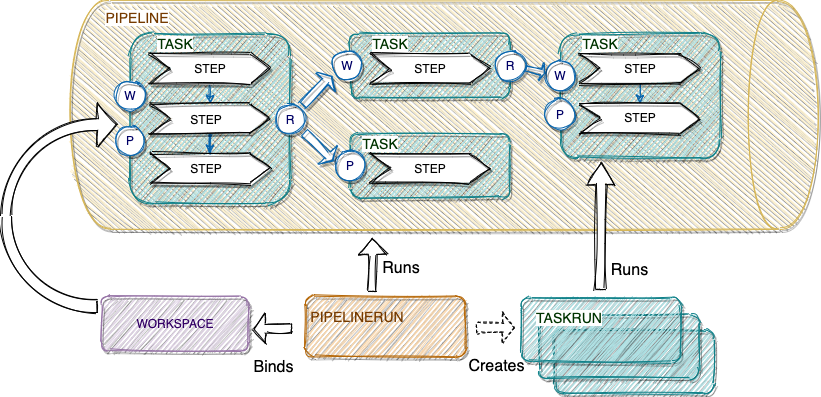
\includegraphics[width=0.5\paperwidth]{img/tekton-workspaces.png}
  \end{textblock*}
\end{lgrayrwhiteframe}

\note{
  Tekton was one of the founding members of the continuous delivery foundation (CDF)
  back at the beginning of 2019.
  It extends the k8s API with CD specific resources.
  Tasks, Pipelines...
  We aim for the Q1 or 2022 for Tekton v1
  Tekton is often used as building block for other platforms, like OpenShift Pipelines,
  Jenkins X, Kubeflow Pipelines and more. The Tekton community cares deeply
  about the stability of its API and happiness of its users.
}

\section[From 0 to Tekton]{From 0 to Tekton\\\ldots step by step}
\begin{sectionwithpic}[cat-walking-on-stairs.jpg]{Public domain photo, CC0}
\end{sectionwithpic}

\note{
  Let's see Tekton in action.
  For the demo sections today, we'll use OpenShift Pipelines, which is a distribution
  of Tekton nicely integrated in OpenShift.
}

\begin{lpicrblack}[nadi-whatisdelirium-fZ8uf_L52wg-unsplash.jpg]{%
  Photo by \href{https://unsplash.com/@whatisdelirium}{\underline{Nadi Whatisdelirium}}, CC0
  }%
  {%
  \begin{itemize}
    \item One-liner (almost)
    \item Tekton Operator (\href{https://operatorhub.io/operator/tektoncd-operator}{\underline{OperatorHub}})
    \item Nightly Builds (Operator too) 
    \item \href{https://cloud.redhat.com/learn/topics/ci-cd}{OpenShift Pipelines} \\~
    \item Multi-architecture (amd64, s390x, ppc64le, arm64)
    \item Multi-OS (Workloads can run on Windows/amd64)
  \end{itemize}
  ~
  \begin{itemize}
    \item Let's install it!
  \end{itemize}
  }%
  {0.42}%
  \frametitle{~~~~~~~~~~~~~~~~~~~~~~~~~~~~~~~~~~~~~~~~~~~~~~~~~~Install}
\end{lpicrblack}

\note{
  First thing, we need to install Tekton.
  There are several options, from a simple one-liner command with kubectl to
  an operator. Tekton can run on several different architectures. It is also
  possible to run Tekton Tasks on Windows cluster nodes.

  OpenShift supports an operator.
  -> Show installing openshift
}

\begin{lgrayframerpic}[thom-milkovic-FTNGfpYCpGM-unsplash.jpg]{%
  Photo by \href{https://unsplash.com/@thommilkovic}{\underline{Thom Milkovic}}, CC0
  }%
  {%
  \begin{itemize}
    \item Tasks \& Pipelines \faProjectDiagram
    \item Parameters, Results \& Workspaces \\~
    \item Catalog \& Hub \faSearch
    \item Git, OCI Registries \\~
    \item Trusted Resources \faLock
  \end{itemize}
  ~
  \begin{itemize}
    \item Let's install some tasks and pipelines
  \end{itemize}
  }%
  {0.48}
  \frametitle{Authoring}
\end{lgrayframerpic}

\note{
  Tekton Tasks and Pipelines are k8s resources, written in YAML.
  The community maintains a catalog of common tasks that can be used
  to compose a pipeline. Organisations may maintain their own catalog too.
  Parameters, workspaces and results represent the interface of both
  tasks and pipelines.

  Pipelines and Tasks can also be stored in container registries.
  The Tekton community is working towards making it easy to sign and
  verify the workflow definitions.

  Show the hub UI, search for a git task
  Search and install git-clone task via tkn
     tkn hub search git-clone
     tkn hub info task git-clone
     tkn hub install task git-clone
     tkn task describe git-clone
     tkn hub install task pylint
     tkn hub install task pytest

  Install other resources via kubectl
     kubectl create -k tekton/

  Start the pipeline via the UI
}

\begin{lpicrblack}[john-yunker-Z9rKuPEU6Uc-unsplash.jpg]{%
  Photo by \href{https://unsplash.com/@jyunker}{\underline{John Yunker}}, CC0
  }%
  {%
  \begin{itemize}
    \item Running Tasks \& Pipelines
  \end{itemize}
  ~\\
  \begin{itemize}
    \item Tekton Dashboard
    \item \code{tkn}, \code{kubectl}
    \item Pods, Volumes \& Events
  \end{itemize}
  ~
  \begin{itemize}
    \item OpenShift Console
  \end{itemize}
  }%
  {0.50}%
  \frametitle{~~~~~~~~~~~~~~~~~~~~~~~~~~~~~~~~~~~~~~~~~~~~~~~~~~~~~~~~~~~~~Watching}
\end{lpicrblack}

\note{
  While the pipeline run, there a few ways we can watch it, starting from
  the OpenShift console itself.
  Since Tekton resources are k8s resources, you can watch them with kubectl
  or tkn.

     tkn pr list
     tkn tr list
     tkn tr describe <tr>
     tkn tr logs <tr>
     kubectl describe tr/<tr>

  And there you can see events too.
  Let's switch back to the console.

  Oh, there was an issue with the snyk check, it looks like the Flask
  version we're using is vulnerable.
  Let's fix it.
  # Create a commit
  Before I push this, I'd like to re-run the pipeline before the PR is merged
  Let's see how we can do that.
}


\begin{lgrayframerpic}[pouncing-cat.png]{Public domain photo, CC0}%
  {%
  \begin{itemize}
    \item Tekton Triggers
    \item Setting up a\\Webhook
    \item Filtering with\\Interceptors
    \item Filtering with\\When Expressions
  \end{itemize}
  }%
  {0.30}
  \frametitle{Launching}
\end{lgrayframerpic}

\note{
  Tekton triggers introduces a few extra k8s custom resources, that can
  be used to listen for events, filter them and run Tekton pipelines as
  a response.
  Let's see how we can set them it up with OpenShift Pipelines.
  # Set it up in OCP
  # Set it up in https://github.com/afrittoli/zero\_to\_tekton/settings
  Now create the PR and watch the pipeline running.
}

\begin{lpicrblack}[sereja-ris-g3B53PbBfwU-unsplash.png]{%
  Photo by \href{https://unsplash.com/@serejaris}{\underline{Sereja Ris}}, CC0
  }%
  {%
  \begin{itemize}
    \item Unattended Execution
    \item Events, \code{CloudEvents}
    \item Notifications:\\GitHub, Slack and more
    \item Monitoring \& Measuring
  \end{itemize}
  ~\\
  \begin{itemize}
    \item Hermetic Builds (Alpha)
    \item Tekton Chains
  \end{itemize}
  }%
  {0.65}%
  \frametitle{~~~~~~~~~~~~~~~~~~~~~~~~~~~~~~~~~~~~~~~~~~~~~~~~~~~~~~~~~~~~~~~~~~~~~~~~~~~~~~~~~~~~Monitoring \& Security}
\end{lpicrblack}

\note{
  It nice to watch your pipeline running, but you many not be always there.
  Tekton can generate events and cloud events that can be used to setup
  notifications and collect data to measure your pipelines.
  Tekton also generates metrics that can be scrapped with Prometheus and
  graphed for instance with Grafana.

  In terms of security Tekton has an alpha version of hermetic builds, which
  isolate specific tasks from the external world. Tekton chains provides out
  band signature of container images and creation of attestations.

  Show the docker hub repo with the signature.
  Check the signature:
     cosign verify -key cosign.pub index.docker.io/andreaf76/zero2tekton:<tag>

  Get the sha from the pipeline results to show the attestation:
     rekor-cli search --sha <sha>
     rekor-cli get --uuid <uuid>
}

\begin{2columnsframe}{Experiments \& Dogfooding}%
  {%
  \begin{itemize}
    \item Custom Tasks:\\
          Loops \& Iterations \\
          Pipeline in Pipelines
          Wait, CEL Run
  \end{itemize}
  ~\\
  ~\\
  ~\\
  ~\\
  \begin{itemize}
    \item Custom Interceptors (GitHub)
    \item DSL, SDK, Notifiers
  \end{itemize}
  }{%
  \begin{itemize}
    \item Using Tekton to CD Tekton
    \item Release, GitOps, CI \\~
  \end{itemize}
  ~\\
  ~\\
  ~\\
  ~\\
  \begin{itemize}
    \item From Experiments to Feature
    \item Source of examples
    \item Bug discovery, feature requests
  \end{itemize}
  }
\end{2columnsframe}

\section[Roadmap]{Roadmap \faRobot\faCat}
\begin{sectionwithpicrx}[julie_falk_flickr_22258190324_6a583208ae_k.png]{Photo by \href{https://www.flickr.com/photos/piper/}{\underline{Julie Falk}}, CC BY-NC 2.0}
\end{sectionwithpicrx}


\begin{2columnsframe}{Roadmap \& Vision}%
  {%
  Mission:
  \begin{itemize}
    \item Be the industry-standard,\\
          cloud-native CI/CD platform \\
          components and ecosystems \\
  \end{itemize}
  ~\\
  ~\\
  \tiny~\\
  \normalsize
  Vision:
  \begin{itemize}
    \item Tekton API conformance across\\
          as many CI/CD platforms as possible
  \end{itemize}
  }{%
  Vision:
  \begin{itemize}
    \item A rich catalog of high quality,\\
          reusable Tasks which work\\
          with Tekton conformant systems\\
  \end{itemize}
  ~\\
  ~\\
  \tiny~\\
  \normalsize
  Roadmap 2021:
  \begin{itemize}
    \item Towards GA, LTS Policies
    \item Security: Audit and Features
    \item User stories, Documentation
    \item Dogfooding
  \end{itemize}
  }
\end{2columnsframe}

\section[Q\&A]{Thank You! \\Questions?}

\begin{sectionwithpiclargecentral}[carl-jorgensen-5nrnxx_tWe8-unsplash.jpg]{Brecon Beacons, Walse, Photo by \href{https://unsplash.com/@scamartist}{\underline{Carl Jorgensen}}, CC0}
\end{sectionwithpiclargecentral}

\begin{blackframe}
  \frametitle{References}
  \begin{itemize}
    \item \large Come and Join Us at Tekton!
    \item \normalsize Tekton community: \href{https://github.com/tektoncd/community}{github.com/tektoncd/community} \\
  \end{itemize}
  \begin{itemize}
    \item Slides: \href{https://github.com/afrittoli/zero_to_tekton/blob/cnd2021/zero_to_tekton.pdf}{github.com/afrittoli/zero\_to\_tekton}
    \item Tekton: \href{https://tekton.dev}{tekton.dev}
    \item Tekton Docs: \href{https://tekton.dev/docs}{tekton.dev/docs}
    \item Tekton on GitHub: \href{https://github.com/tektoncd}{github.com/tektoncd}
    \item Tekton Hub: \href{https://hub.tekton.dev}{hub.tekton.dev}
    \item Tekton on Operator Hub:\\\href{https://https://operatorhub.io/operator/tektoncd-operator}{https://operatorhub.io/operator/tektoncd-operator}
    \item Tekton Results: \href{https://github.com/tektoncd/results}{github.com/tektoncd/results}
    \item Tekton Enhancement Proposals (TEPs): \href{https://github.com/tektoncd/community/tree/main/teps\#tekton-enhancement-proposals-teps}{github.com/tektoncd/community/tree/main/teps}
  \end{itemize}
  \begin{textblock*}{0.13\paperwidth}(0.73\paperwidth,0.65\paperheight)
    \includesvg[width=0.13\paperwidth]{img/tekton-icon-color.svg}
  \end{textblock*}
\end{blackframe}

\end{document}
